\documentclass[10pt, conference]{FMFP2022}
% \documentclass[10pt]{article}
% \usepackage[top=1.50cm, bottom=1.50cm, left=1.884cm, right=1.884cm, includehead, includefoot, heightrounded]{geometry}
\usepackage{fancyhdr} % To use headers
\usepackage{graphicx} %To use graphics package
\usepackage[textfont=bf, font = normalsize]{caption} %To use bold and normal size font for table and figure captions
% \usepackage{floatrow} %To have table captions above the table
\usepackage{float}
\usepackage{amssymb}
\usepackage{amsfonts}
\usepackage{amsmath}
\floatstyle{plaintop} %To have table captions above the table
\restylefloat{table} %To have table captions above the table
\usepackage{subfigure} % To use subfigures
 % \floatsetup{font = normalsize} %Size of font in tables

\rhead{
    \sffamily\fontsize{9}{11}\selectfont
    \vspace{-0.5cm}
    \textbf{Proceedings of the 9th International and 49th National Conference on
      Fluid Mechanics and Fluid Power (FMFP) \\ December 14-16, 2022, IIT
      Roorkee, Roorkee-247667, Uttarakhand, India} \\ \vspace{0.15cm}
    \large{\textbf{FMFP2022-12-2022}}}

  % \vspace{1cm}


\usepackage{hyperref}
\usepackage{graphicx}
% \usepackage{subcaption}
\usepackage{amssymb}
\usepackage{amsmath}
\usepackage{multirow}
\usepackage{relsize}
\usepackage[utf8]{inputenc}
\usepackage{cleveref}
\usepackage{algorithm}
\usepackage[noend]{algpseudocode}
\usepackage[section]{placeins}
\usepackage{booktabs}
\usepackage{url}
\usepackage{microtype}

% For the TODOs
\usepackage{xcolor}
\usepackage{xargs}
\usepackage[colorinlistoftodos,textsize=footnotesize]{todonotes}
\newcommand{\todoin}{\todo[inline]}
% from here: https://tex.stackexchange.com/questions/9796/how-to-add-todo-notes
% \newcommandx{\unsure}[2][1=]{\todo[linecolor=red,backgroundcolor=red!25,bordercolor=red,#1]{#2}}
% \newcommandx{\change}[2][1=]{\todo[linecolor=blue,backgroundcolor=blue!25,bordercolor=blue,#1]{#2}}
% \newcommandx{\info}[2][1=]{\todo[linecolor=OliveGreen,backgroundcolor=OliveGreen!25,bordercolor=OliveGreen,#1]{#2}}

%Boldtype for greek symbols
\newcommand{\teng}[1]{\ensuremath{\boldsymbol{#1}}}
\newcommand{\ten}[1]{\ensuremath{\mathbf{#1}}}

\usepackage{lineno}


\renewcommand{\headrulewidth}{0pt}


\begin{document}

\title{\LARGE{ \bf Fluid-Structure Interaction with an Updated
    Lagrangian Smoothed Particle Hydrodynamics }}
\author{\textbf{Dinesh Adepu\textsuperscript{1}, Prabhu Ramachandran\textsuperscript{1}}\\\\
  \textsuperscript{1}\small{Department of Aerospace Engineering, Indian
    Institute of Technology Bombay, Powai, Mumbai 400076, India}}

\maketitle
\thispagestyle{fancy}
\pagestyle{plain} % To suppress headers but still include page numbers from second page on

\noindent \textbf{ABSTRACT}
A corrected transport velocity formulation (CTVF) based solver is developed to
study the deformation of elastic structures under hydrodynamic loads. CTVF is
adopted to handle both fluid and structural dynamics. The current solver’s
advantage is to eliminate inhomogeneous particle distribution in fluid flow and
tensile instability in elastic structures. A ghost particle-based approach is
used to handle the coupling between the fluid and solid phases. The proposed
scheme is verified by simulating a few test cases, which we validate with exact
analytical solutions. As an application, we simulate an elastic plate
deformation due to dam-breaking fluid.\noindent\\
\textbf{Keywords:} Smoothed particle hydrodynamics; Fluid-structure interaction; Transport velocity formulation \\

\section{{\textbf{INTRODUCTION}}}
Fluid-structure interaction (FSI) is a common engineering problem that is seen
in daily life. Some examples include the deformation of the wind turbine blade
due to the fluid flow, the flow traversal due to the deflected blade, blood flow
in heart value, coastal engineering, and vortex-induced vibration
\cite{williamson2004vortex,bearman2011circular}. An accurate study of FSI can
allow us to optimize the systems where FSI is dominant. However, studying the
FSI phenomena through experiments or analytical techniques is complex due to its
nonlinear behavior. % Therefore, a computational study is preferred which
% comprises of mesh-based and meshless methods.
% \todo{Re-write}

Mesh-based schemes such as finite element method (FEM)
\cite{lozovskiy2015unconditionally} and finite volume method (FVM)
\cite{jasak2007updated} have been used for the last few decades in modeling the
FSI problems. However, mesh-based methods are not favorable when dealing with
free surface flow problems or problems involving large deformation of the
structure. This is due to explicit free surface tracking, and mesh distortion
\cite{moresi2003lagrangian} while dealing with large deformation solids.
Therefore, meshless methods are preferred while handling FSI problems involving
free surfaces, multiphase flows, and large deformation in solids. The smoothed
particle hydrodynamics (SPH) and material point method (MPM) are more commonly
used to model the fluid phase. While the solids are modeled with SPH or
Reproducing Kernel Particle Methods (RKPM), or the Discrete Element Method (DEM)
\cite{hu2010material,li2022material}. These meshless techniques have been
coupled for the past two decades to model the fluid-structure interaction. A few
schemes with SPH and MPM are SPH-DEM~ \cite{wu2016coupled},
SPH-TLSPH~\cite{salehizadeh2022coupled}, SPH-RKPM~\cite{peng2021coupling},
SPH-Peridynamics~\cite{sun2020smoothed}, MPM-DEM~\cite{singer2022partitioned}.
For more, see the review by \cite{khayyer2022systematic}. In the current work,
we use SPH to handle FSI problems.


In SPH, fluids are modeled primarily using two approaches, one by assuming they
are weakly compressible and another by considering them incompressible. Though
SPH is successful in modeling fluid flows, it suffers from particle pairing and
irregular particle distribution problems resulting in poor function
approximation~\cite{rastelli2022implicit} and unstable simulations. To
homogenize the particles, \cite{xu2009accuracy} adjusts the particle positions
after each timestep. Then, the particle properties are adjusted to the new
position using Taylor series approximation. Later, Adami \cite{adami2013transport}
proposed a transport velocity formulation (TVF) scheme where the particles are
moved with a "transport velocity" rather than the momentum velocity. TVF is
applied to internal fluid flow problems. Zhang
\cite{zhang2017generalized} extended the TVF formulation and called it the
generalized TVF (GTVF) and applied it to free surface problems and elastic
solids. However, while extending TVF, GTVF has missing terms and is sensitive to
the particle shifting technique (PST). \cite{adepu2021corrected} proposed a
corrected TVF (CTVF) scheme where the missing terms in TVF are incorporated and
is robust to the PST. While handling elastic solids with SPH, the classical
SPH~\cite{gray2001sph} faces tensile instability and results in numerical
fracture. \cite{gray2001sph} has proposed adding artificial stress,
~\cite{chalk2020stress} introduces stress-points in addition to the existing
particles, \cite{sugiura2017extension} modifies the equation of state to
eliminate the tensile instability. CTVF can eliminate tensile instability and
handle higher Poisson ratios. While CTVF is also robust to different PST. FSI in
SPH is modeled by several works, such as, WCSPH-Total Lagrangian SPH (TLSPH)
\cite{zhan2019stabilized}, WCSPH-Updated Lagrangian SPH (ULSPH)
\cite{antoci2007numerical}, ISPH-TLSPH\cite{salehizadeh2022coupled}.

Handling FSI problems with the transport velocity formulation framework is
advantageous as it can solve the tensile instability issue in solid dynamics and
inhomogeneous particle distribution in fluids. In the current work, we handle
FSI problems by the CTVF method, where both fluids and solid phases are modeled
using CTVF alone. To validate the proposed method, we consider three numerical
test cases. A uniformly distributed load over a clamped beam (UDL) problem is
considered to validate the elastic dynamics of CTVF. An aluminum plate over a
hydrostatic tank for FSI validation is considered. Finally, it is applied to a
fluid flow hitting an elastic plate. Here, the deformation of the elastic
plate is compared against the experimental results. A convergence analysis is
undertaken for both UDL and elastic deformation under hydrodynamic load
problems.

\section{\textbf{METHODOLOGY}}\label{sec2}

We follow CTVF formulation to model the fluid and solid phase. Following CTVF,
the particles are moved with a transport velocity rather than the momentum
velocity, with which we get a homogenized particle distribution as well as it
eliminates the tensile instability. In the next two sections we show the
discretized equations of both fluid and solid phase. Please see
\cite{adepu2021corrected} for more details.

\subsection{\textbf{Discrete equations of the fluid medium}}\label{subsec:discrete-fluid}

The governing equations of the fluid are conservation of mass and momentum.
Following the weakly compressible SPH scheme, we use an equation of state to
complete the system. The SPH discretization of the continuity
equation~\eqref{eq:sph-discretization-continuity} and the EDAC
based~\cite{PRKP:edac-sph-iccm2015} pressure evolution
equation~\eqref{eq:sph-discretization-edac} respectively are,
\begin{equation}
  \label{eq:sph-discretization-continuity}
  \frac{\tilde{d}\rho_a}{dt} = \sum_{b} \; \frac{m_b}{\rho_{b}} \; (
  \rho_{a} \; \tilde{\ten{u}}_{ab} \; + \;
  (\rho \; (\tilde{\ten{u}} \; - \;
  \ten{u}))_{ab}) \; \cdot \nabla_{a} W_{ab},
\end{equation}
\begin{multline}
  \label{eq:sph-discretization-edac}
  \frac{\tilde{d}p_a}{dt} = \sum_{b} \; \frac{m_b}{\rho_{b}} \; \bigg(
  (p_{a} - \rho_{a} c_{s}^2) \; \ten{u}_{ab} \; + \;
  p_{a} \; \tilde{\ten{u}}_{ab} \; - \;
  (p \; (\tilde{\ten{u}} - \ten{u}))_{ab} \; + \; \\
  4 \; \nu_{edac}
  \frac{p_a - p_b}{(\rho_a + \rho_b) (r^2_{ab} + 0.01 h_{ab}^{2})} \ten{r}_{ab}
  \bigg) \; \cdot \nabla_{a} W_{ab}.
\end{multline}
%
Where $\frac{\tilde{d}}{dt}$ is the material derivative, with $\tilde{u}$ being
the transport velocity of the particles, $\ten{u}_{ab} = \ten{u}_a - \ten{u}_b$.
%
Similarly, the discretized momentum equation for fluids is written as,
\begin{multline}
  \label{eq:sph-momentum-fluid}
  \frac{\tilde{d}\ten{u}_{a}}{dt} = - \sum_{b} m_b \bigg[
  \bigg(\frac{p_a}{\rho_a^2} + \frac{p_b}{\rho_b^2}\bigg) \ten{I} -
  \bigg(\frac{\ten{A}_a}{\rho_a^2} + \frac{\ten{A}_b}{\rho_b^2} + \Pi_{ab}
  \ten{I} \bigg) \bigg]
  \cdot \nabla_{a} W_{ab} \\
  + \ten{u}_{a} \sum_{b} \frac{m_b}{\rho_{b}} \; \tilde{\ten{u}}_{ab} \cdot
  \nabla_{a} W_{ab} \\+ \sum_{b} m_b \frac{4 \eta \nabla W_{ab}\cdot
    \ten{r}_{ab}}{(\rho_a + \rho_b) (r_{ab}^2 + 0.01 h_{ab}^2)} \ten{u}_{ab} +
  \ten{g}_{a} + \frac{\ten{F}^a_{\text{FSI}}}{m_a}
\end{multline}
where $\ten{A}_a = \rho_a \ten{u}_a \otimes (\ten{\tilde{u}}_a - \ten{u}_a)$,
$\ten{I}$ is the identity matrix, $\eta$ is the kinematic viscosity of the
fluid and \cite{morris-lowRe-97} formulation is used to discretize the
viscosity term. $\Pi_{ab}$ is the artificial
viscosity~\cite{monaghan-review:2005} to maintain the stability of the
numerical scheme. It is given as,
\begin{align}
  \label{eq:mom-av}
  \Pi_{ab} =
  \begin{cases}
\frac{-\alpha h_{ab} \bar{c}_{ab} \phi_{ab}}{\bar{\rho}_{ab}}
  & \ten{u}_{ab}\cdot \ten{r}_{ab} < 0, \\
  0 & \ten{u}_{ab}\cdot \ten{r}_{ab} \ge 0,
\end{cases}
\end{align}
where,
%
\begin{equation}
  \label{eq:av-phiij}
  \phi_{ab} = \frac{\ten{u}_{ab} \cdot \ten{r}_{ab}}{r^2_{ab} + 0.01 h^2_{ab}},
\end{equation}
%
where, $\ten{r}_{ab} = \ten{r}_a - \ten{r}_b$, $h_{ab} = (h_a + h_b)/2$,
$\bar{\rho}_{ab} = (\rho_a + \rho_b)/2$, $\bar{c}_{ab} = (c_a + c_b) / 2$, and
$\alpha$ is the artificial viscosity parameter. $\ten{F}^a_{\text{FSI}}$ is the
force due to the interaction with elastic structure. This force modeling is
explained in \cref{subsec:fsi}. We utilize the ghost particle approach proposed
in \cite{Adami2012} to handle the boundaries.



\subsection{\textbf{Solid phase modeling}}\label{subsec:solid}
Similar to discretized fluid governing equation, the elastic structure equations are
\eqref{eq:sph-discretization-continuity}, and the momentum equation,
\begin{multline}
  \label{eq:sph-momentum-solid}
  \frac{\tilde{d}\ten{u}_{a}}{dt} = - \sum_{b} m_b \bigg[
  \bigg(\frac{p_a}{\rho_a^2} + \frac{p_b}{\rho_b^2}\bigg) \ten{I} -
  \bigg(\frac{\teng{\sigma}^{'}_{a}}{\rho_a^2} +
  \frac{\teng{\sigma}^{'}_{b}}{\rho_b^2} + \Pi_{ab} \ten{I} \bigg) \bigg]  \cdot \nabla_{a} W_{ab} \\
  + \ten{g}_{a} + \frac{\ten{F}^a_{\text{FSI}}}{m_a},
\end{multline}
while the additional stress terms, $\ten{A}$ in momentum equation of solid
mechanics are not considered as it has a negligible effect. An equation of state
is utilized to link the pressure with density following a weakly compressible
SPH scheme. Jaumann stress rate equation is solved to evolve the shear stress,
given as,
\begin{multline}
  \label{eq:sph-modified-jaumann-stress}
  \frac{\tilde{d}\teng{\sigma}^{'}_{a}}{dt} = 2G (\dot{\teng{\epsilon}}_{a} -
  \frac{1}{3} \dot{\teng{\epsilon}}_{a} \ten{I}) + \teng{\sigma}^{'}_{a}
  \teng{\Omega}_{a}^{T} +
  \teng{\Omega}_{a} \teng{\sigma}^{'}_{a}
\end{multline}
The SPH discretization of the
gradient of velocity is given as,
\begin{equation}
  \label{eq:sph-vel-grad}
  \nabla \ten{u}_a =
  - \sum_{b} \frac{m_b}{\rho_{b}} (\ten{u}_{a} - \ten{u}_{b}) \otimes (\nabla_{a} W_{ab}),
\end{equation}
where $\otimes$ is the outer product. With the strain and rotation tensors as,
\begin{equation}
  \label{eq:strain-tensor}
  \dot{\epsilon}_{ij} = \frac{1}{2} \bigg(\frac{\partial u_i}{\partial x_j} +
  \frac{\partial u_j}{\partial x_i} \bigg),
\end{equation}
and $\Omega_{ij}$ is the rotation tensor,
\begin{equation}
  \label{eq:rotational-tensor}
  \Omega_{ij} = \frac{1}{2} \bigg(\frac{\partial u_i}{\partial x_j} -
  \frac{\partial u_j}{\partial x_i} \bigg).
\end{equation}


\subsection{\textbf{Transport velocity computation}}\label{subsec:transport-velocity}
The particles in the current scheme are moved with the transport velocity,
\begin{equation}
  \label{eq:transport_velocity_position_derivative}
  \frac{d\ten{r}_a}{dt} = \ten{\tilde{u}}_a.
\end{equation}
%
The transport velocity is updated using,
\begin{equation}
  \label{eq:transport_velocity}
  \ten{\tilde{u}}_a(t + \Delta t) =\ten{u}_a(t) + \Delta t \; \frac{\tilde{d} \ten{u}_a}{dt} +
  \bigg(\frac{d \ten{u}_{a}}{dt}\bigg)_{\text{c}} \Delta t
\end{equation}

Where $\big(\frac{d \ten{u}_a}{dt}\big)_{\text{c}}$ is the homogenization
acceleration which ensures that the particle positions are homogeneous. In the
current work we have used Sun's \cite{sun_consistent_2019} PST to homogenization
the fluid medium while iterative PST (IPST)\cite{huang_kernel_2019} for the
solid phase. According to \cite{adepu2021corrected} the force formulation of
\cite{sun_consistent_2019} is,
\begin{equation}
  \label{eq:sun2019_pst}
  \bigg(\frac{d \ten{u}_a}{dt}\bigg)_{\text{c}} = - \frac{\text{M} \;
    (2h) c_0}{\Delta t} \sum_b \bigg[1 + R \bigg( \frac{W_{ab}}{W(\Delta x)} \bigg)^n
  \bigg] \nabla_a W_{ab} V_b,
\end{equation}
where $R$ is an adjustment factor to handle the tensile instability, and
$\text{M}$ is the mach number of the flow. $V_b$ is the volume of the
$b$\textsuperscript{th} particle, $c_0$ is the speed of sound. The acceleration is modified to account for
particles on the free surface. Here, $R = 0.2$ and $n = 4$ are used. Please see
\cite{adepu2021corrected} for detailed explanation of PST.

\subsection{\textbf{Fluid-structure interaction}}\label{subsec:fsi}
Coupling is handled in a straight forward way in SPH. While modelling the fluid
phase and treating the fluid-structure interactions, the structure particles are
assumed to be boundary particles. From the boundary handling given in Adami
\cite{Adami2012}, we compute the pressure of the boundary particles from
the extrapolated equation as,
\begin{equation}
  \label{eq:pressure-bc}
  p_s = \frac{\Sigma_f p_f W_{sf} + (\ten{g} - \ten{a}_{\ten{s}}) \cdot \Sigma_f
    \rho_f \ten{r}_{sf} W_{sf}}{\Sigma_f W_{sf}}.
\end{equation}
Here, $\ten{a}_s$ is the acceleration of the structure particles. The subscript
$f$ denotes the fluid particles and $s$ denotes the structure particles. By the
extrapolated pressure, hydrodynamic density of structure properties are
computed. Please note that the pressure we set here are only pertaining to the
FSI force and does not correspond to the real pressure or density of the
structure particles. By utilizing the previously set hydrodynamic properties on
the structure, the interaction force is computed using,
\begin{equation}
  \ten{F}_{\text{FSI}}^i = -m_i \sum_{a} m_a \bigg(\frac{p_i}{\rho_{i}^2} +
  \frac{p_a}{\rho_{a}^2} + \Pi_{ia} \bigg) \nabla_{i} W(x_{ia})
\end{equation}
where $i$ is fluid particle, $a$ is structure particle.


\section{\textbf{RESULTS AND DISCUSSION}}\label{sec3}

% =========================================
% =========================================
% start
% =========================================
% =========================================
\subsection{Uniformly distributed loading (UDL) on a clamped beam}
\label{sec:udl}

In the first test case, we validate the structural part of the current solver.
We chose a homogeneous elastic plate clamped on both ends acted upon by a
uniformly distributed load ($q = 20$ Nm$\textsuperscript{-1}$) as shown in
\cref{fig:udl-schematic}. The beam's length (L) and height (H) is 0.2 m and
\begin{figure}[!htpb]
  \centering
  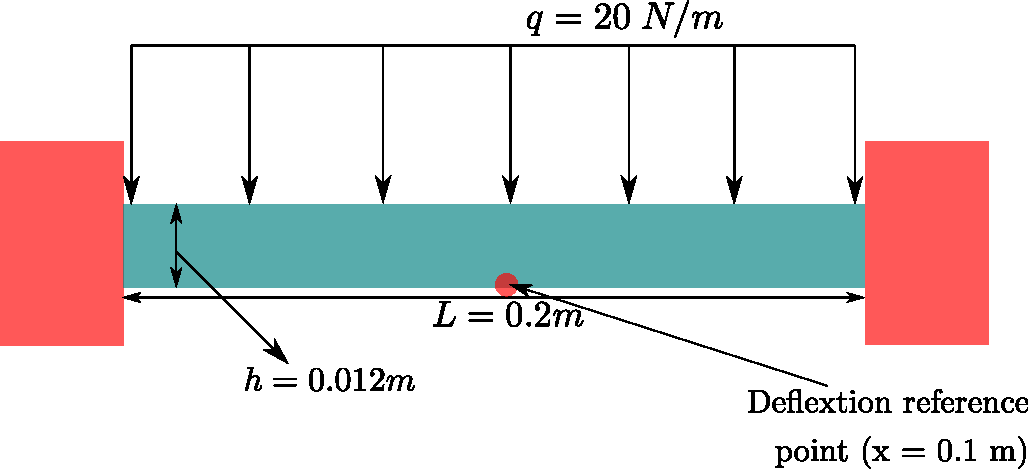
\includegraphics[scale=0.5]{images/khayyer_2021_udl/schematic}
  \caption{The schematic of a clamped elastic beam being acted upon by a
    uniformly distributed load.}
\label{fig:udl-schematic}
\end{figure}
$0.012$ m, respectively. The mechanical properties of the plate are set as
$E=10^7$ Pa in Young's modulus, $\nu=0$ in Poisson's ratio and $\rho=1000$
kgm$\textsuperscript{-3}$) in density. The numerical solution of the
y-displacement at the center of the beam is compared against the analytical
counterpart. The analytical solution for the deflection of a uniformly
distributed beam clamped at both ends is given by
\begin{equation}
  \label{eq:ce-tvf}
  \eta\left(\frac{L}{2}\right) = \frac{qL^4}{384 D},
\end{equation}
where, $D$ is defined as $\frac{E h^3}{12 (1 - (\nu)^2)}$. We consider three
particle resolutions such that, $10$, $15$, and $20$ particles along the beam's
width are used. We run for a total physical time of $2$ seconds.

\Cref{fig:udl-disp-plot} depicts the time history of y-displacement of the beam
center for different particle resolutions computed using the current solver
compared against the analytical solution. From \cref{fig:udl-disp-plot}, we can
see that the current solver can accurately predict the displacement of the
\begin{figure}
  \centering
  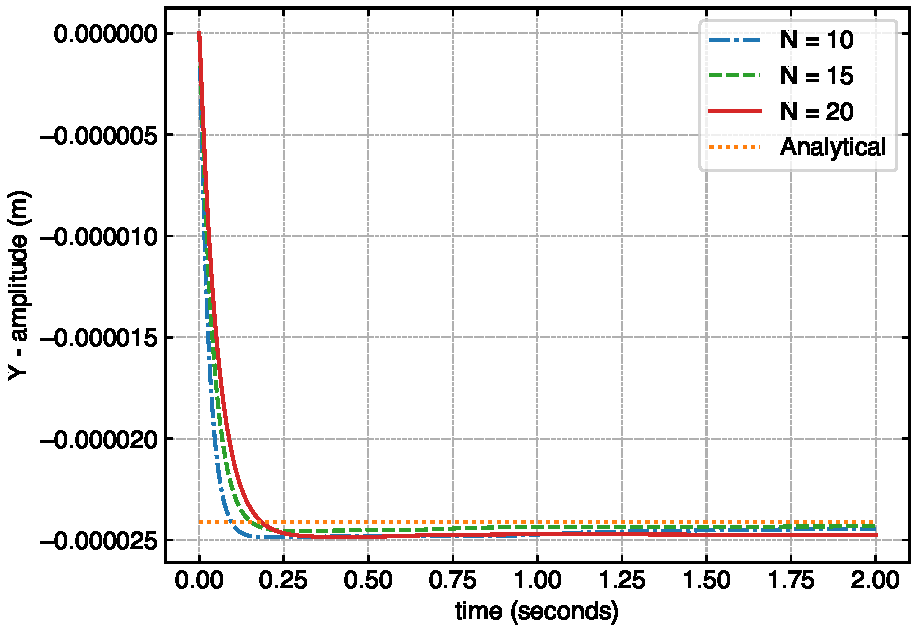
\includegraphics[scale=0.5]{figures/khayyer_2021_udl/homogenous}
  \caption{Time variation of the y-displacement of the center of the beam for
    three different resolutions, compared against the analytical result.}
\label{fig:udl-disp-plot}
\end{figure}
clamped beam. Convergence of the current scheme is captured in
\cref{fig:udl-disp-plot}, and the computational results are within a reasonable
variation of the analytical solution with the variation of the particle spacing.


\subsection{Hydrostatic water column on an elastic plate}
\label{sec:hydrostatic-water-column-on-an-composite-elastic-plate}
In this example we study the deformation of an elastic plate due to the
hydrostatic water column. We utilise the current example to examine the accuracy
and convergence of the current solver. The schematic of fluid with the elastic
beam is shown in \cref{fig:hs-water-on-plate} along with the initial pressure
distribution in the fluid. The figure includes the dimensions as well. The
material properties of the beam are, a density of $2700$
kgm\textsuperscript{-3}, with an Young's modulus of $67.5$ GPa, and a Poisson
\begin{figure}
  \centering
  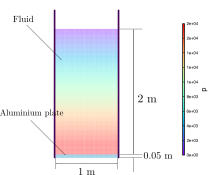
\includegraphics[scale=0.4]{images/ng_2020_hydrostatic_water_column_on_elastic_plate/schematic}
  \caption{Schematic of the hydrostatic water column on an elastic plate. Fluid
    particle color represents pressure.}
\label{fig:hs-water-on-plate}
\end{figure}
ratio of $0.34$. The material properties of the fluid are, a density of $1000$
kgm\textsuperscript{-3}, with a dynamic viscosity of $0$
kgm\textsuperscript{-1}s\textsuperscript{-1}. We consider two particle
resolutions such that we get $10$, $15$ and $20$ particles along the width
directing of the beam. We run the simulation for a total physical time of $3$
seconds. The y-displacement at the center of the beam is compared against the
analytical with the current numerical solver for quantitative validation. Here,
the beam deflection computed using an analytical expression results in a
deflection $d = -6.85 \times 10^{-5}$ m.

\Cref{fig:snapshot-hs-fsi} shows the particle plot of the fluid along with the
elastic solid at time $2$ seconds with color of the fluid particles describing
the pressure. This snapshot corresponds to the highest particle resolution i.e.,
$20$ particles along the width direction. From the \cref{fig:snapshot-hs-fsi},
we can see that the current solver produces a smooth pressure distribution
\begin{figure}
    \centering
    \subfigure
    {
      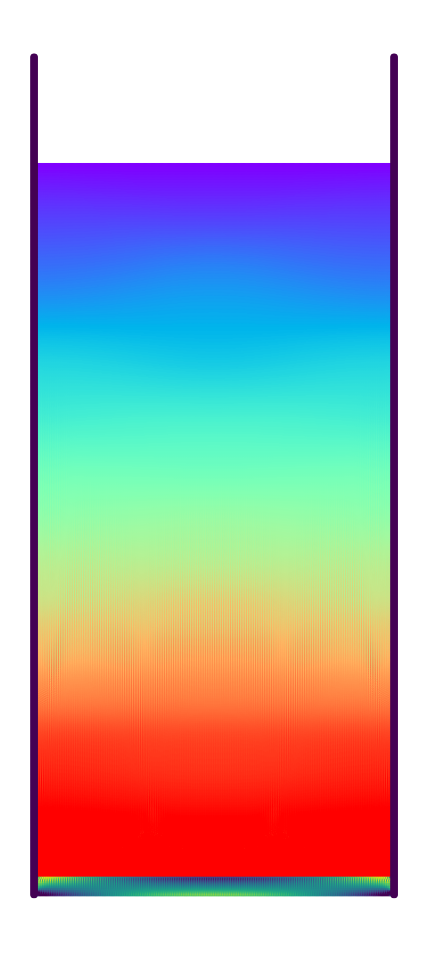
\includegraphics[scale=1.0]{figures/ng_2020_hydrostatic_water_column_on_elastic_plate/snap_t_0}
    }
    \qquad
    \subfigure
    {
      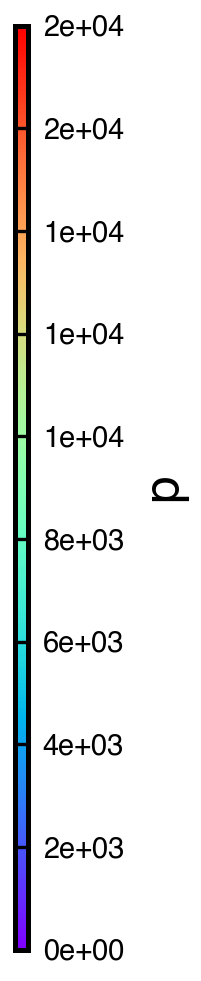
\includegraphics[scale=1.0]{figures/ng_2020_hydrostatic_water_column_on_elastic_plate/colorbar_t_0}
    }
    \caption
    { Snapshot of the fluid and the elastic structure at time 0.5 sec
      including the pressure of the fluid.}
    \label{fig:snapshot-hs-fsi}
\end{figure}
demonstrating the stability of the current solver.
\Cref{fig:ng2020hsplate:deflection} depicts the time history of y-displacement
of the beam center for different particle resolutions computed using the current
solver compared against the analytical solution. From
\cref{fig:ng2020hsplate:deflection} we can see that the current solver is able
to predict the displacement of the clamped beam within the vicinity of the
analytical results. Also as the particle spacing is reduced, the beam
displacement is converging as well.
\begin{figure}
  \centering
  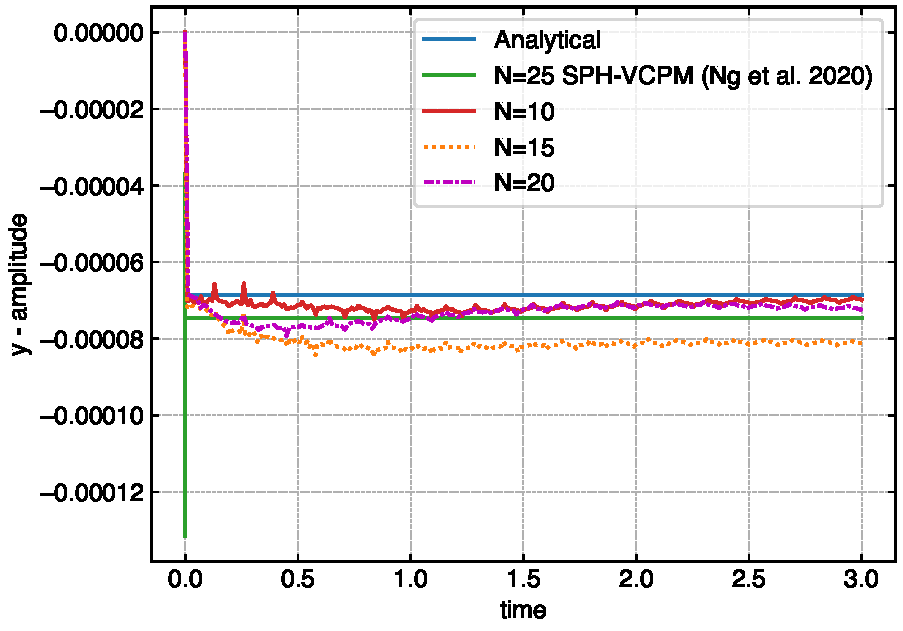
\includegraphics[scale=0.5]{{{figures/ng_2020_hydrostatic_water_column_on_elastic_plate/y_amplitude}}}
  \caption{The mid-span deflection of the structure under hydrodynamic loading
    with time for different resolutions, compared against the analytical and
    the numerical result of \cite{ng2020coupled}}
\label{fig:ng2020hsplate:deflection}
\end{figure}
%


\subsection{Water impact onto an elastic plate}
\label{sec:water-impact-forefront}
In this case, we study the deformation of the elastic plate due to the impact of
a dam breaking flow. \Cref{fig:dam-break-flow-impact-plate-initial-setup} shows
the initial positions of fluid and the structure inside the dam, including the
dimensions. Following \cite{sun2019fully} we set the material properties of the
elastic plate, a density of $2500$ kgm\textsuperscript{-3}, with an Young's
modulus of $10^6$ Pa, and a Poisson ratio of $0$. The material properties of the
fluid are, a density of 1000 kgm\textsuperscript{-3}, with a dynamic viscosity
of 0 kgm\textsuperscript{-1}s\textsuperscript{-1}. A particle spacing of $5$
$\times$ $10^{-4}$ m is taken, resulting in a total of $182911$ particles, which
includes fluid, structure and solid wall. We run a total physical time of $0.7$
seconds. Here the fluid is initially released which attains a certain velocity
by the time it impacts the structure. The structure will obstruct the fluid
making it rise and the fluid will deform the elastic plate. The fluid will rise
and hit the other end of the dam, following it comes back and hits the structure
from the back. For a quantitative validation, we compare the current solver
results to the other numerical techniques.
\begin{figure}
  \centering
  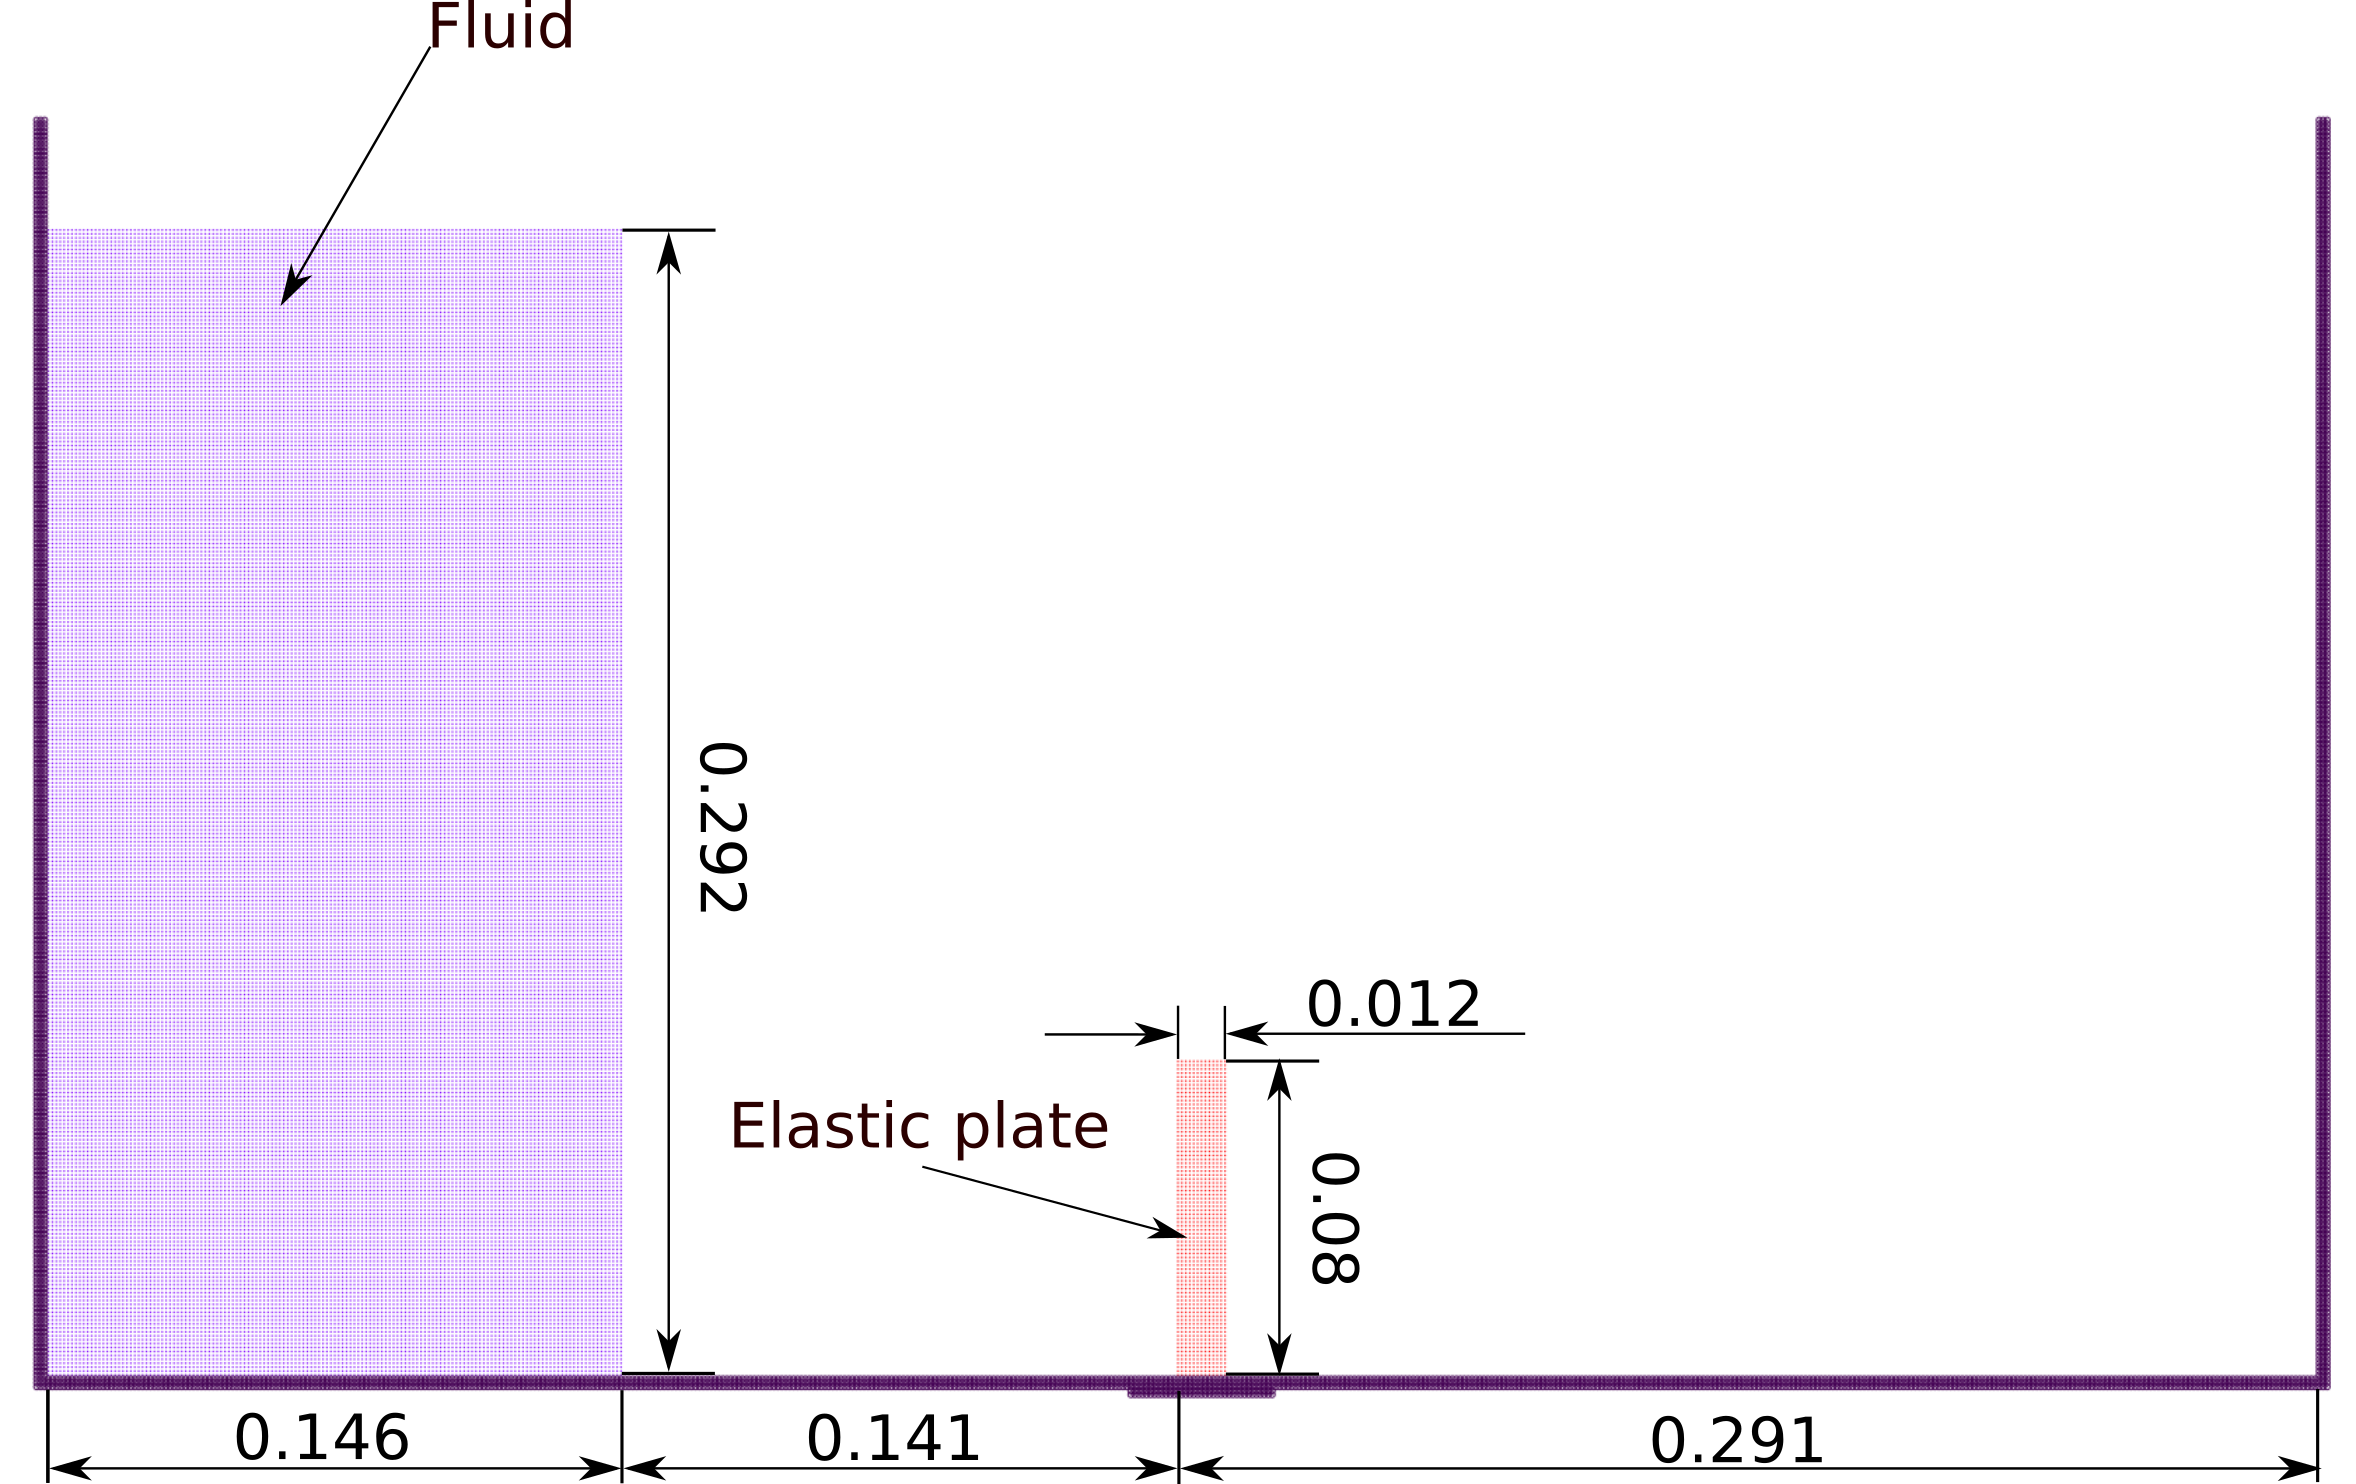
\includegraphics[scale=0.4]{images/sun_2019_dam_breaking_flow_impacting_an_elastic_plate/schematic}
  \caption{Schematic of the dam-break flow impacting an elastic plate. All dimensions are in meters.}
\label{fig:dam-break-flow-impact-plate-initial-setup}
\end{figure}

\Cref{fig:dam-breaking-onto-plate-snapshot} shows the snapshots of the fluid and
the elastic structure at different time instances. From
\cref{fig:dam-breaking-onto-plate-snapshot}, we can see that the fluid after
hitting the structure rises and hits the other end of the tank and travels back
to hit the structure again. The time variation of the x-displacement of the
elastic structure is compared against other numerical
results~\cite{sun2019fully,bogaers2016evaluation}. From the
\cref{fig:water-impact-plate-deflection-quantitative} we can see that the
displacement computed by the current solver is with in a vicinity of the other
results produced.
% \begin{figure}[H]
%     \centering
%     \subfigure[]
%     {
%         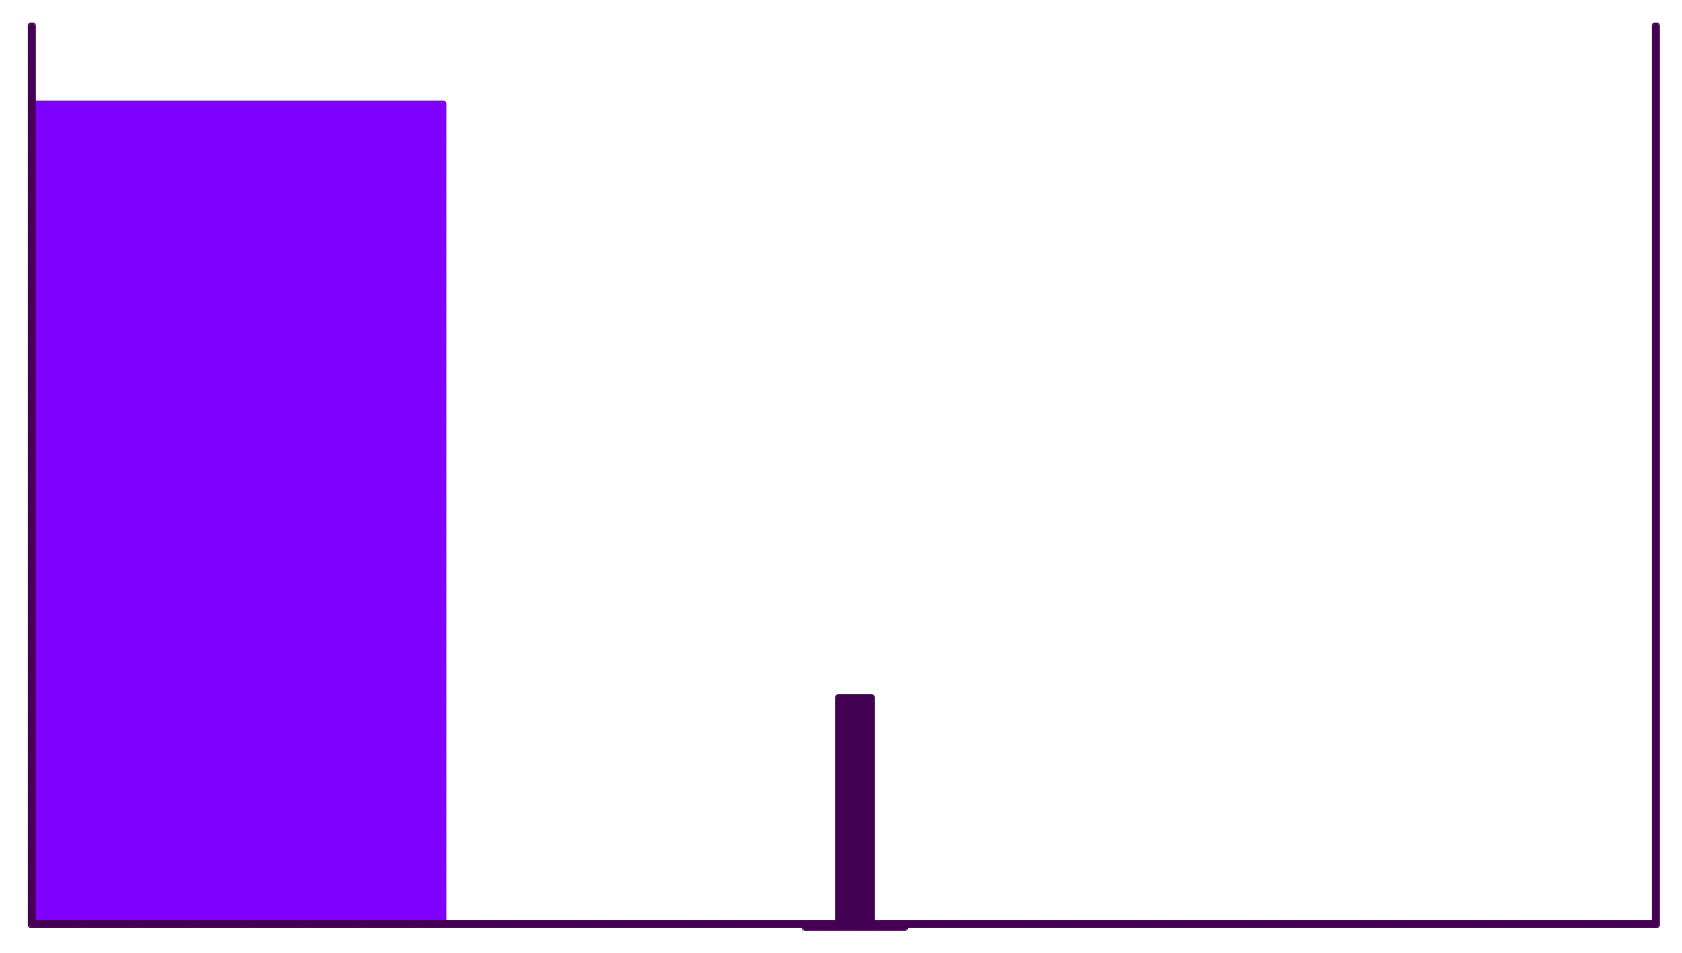
\includegraphics[scale=0.5]{figures/sun_2019_dam_breaking_flow_impacting_an_elastic_plate/snap_t_0.png}
%     }
%     \\
%     \subfigure[]
%     {
%         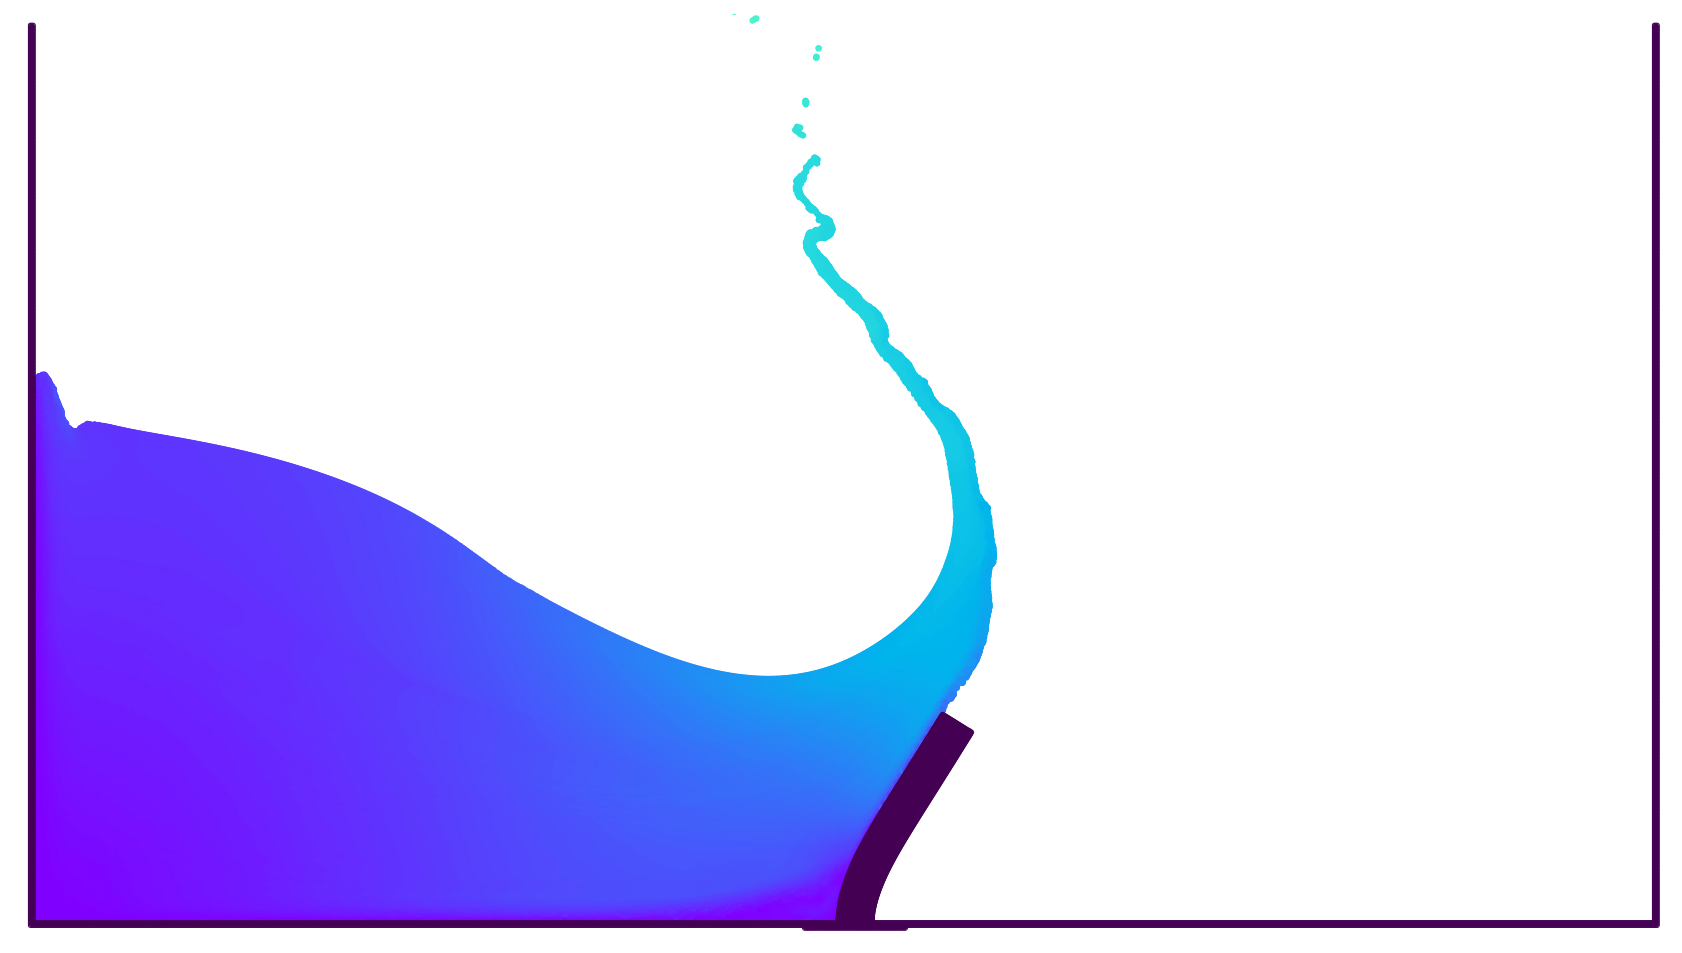
\includegraphics[scale=0.5]{figures/sun_2019_dam_breaking_flow_impacting_an_elastic_plate/snap_t_1.png}
%     }
%     \\
%     \subfigure[]
%     {
%         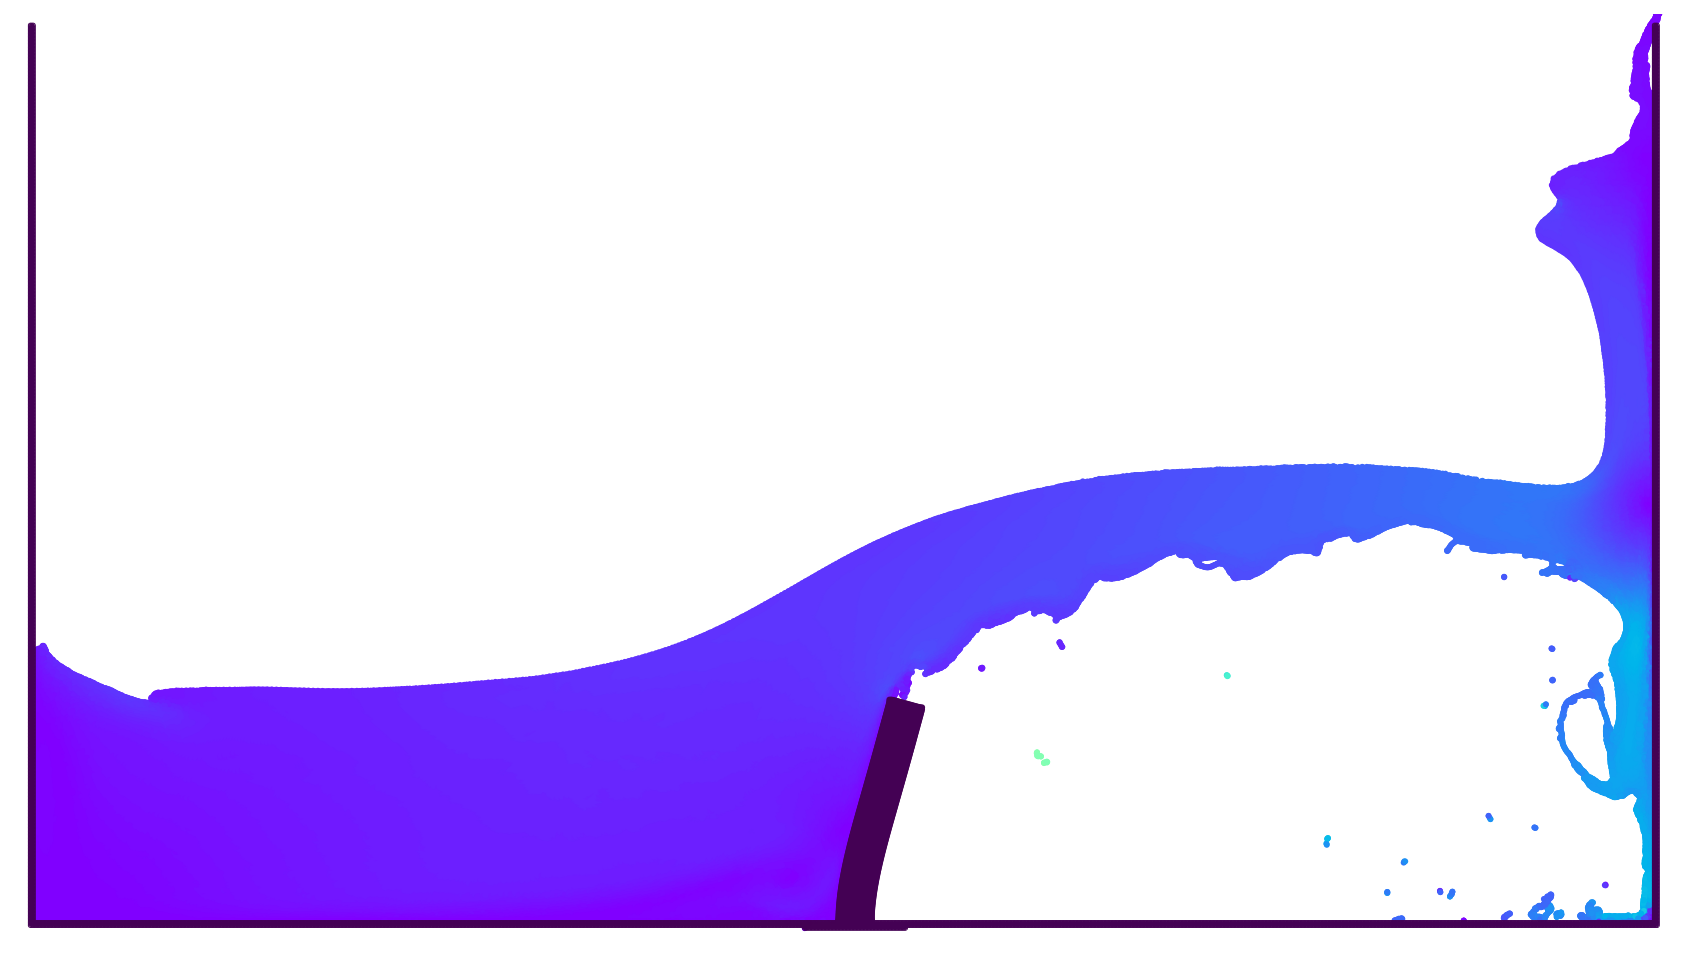
\includegraphics[scale=0.5]{figures/sun_2019_dam_breaking_flow_impacting_an_elastic_plate/snap_t_2.png}
%     }
%     \\
%     \subfigure[]
%     {
%         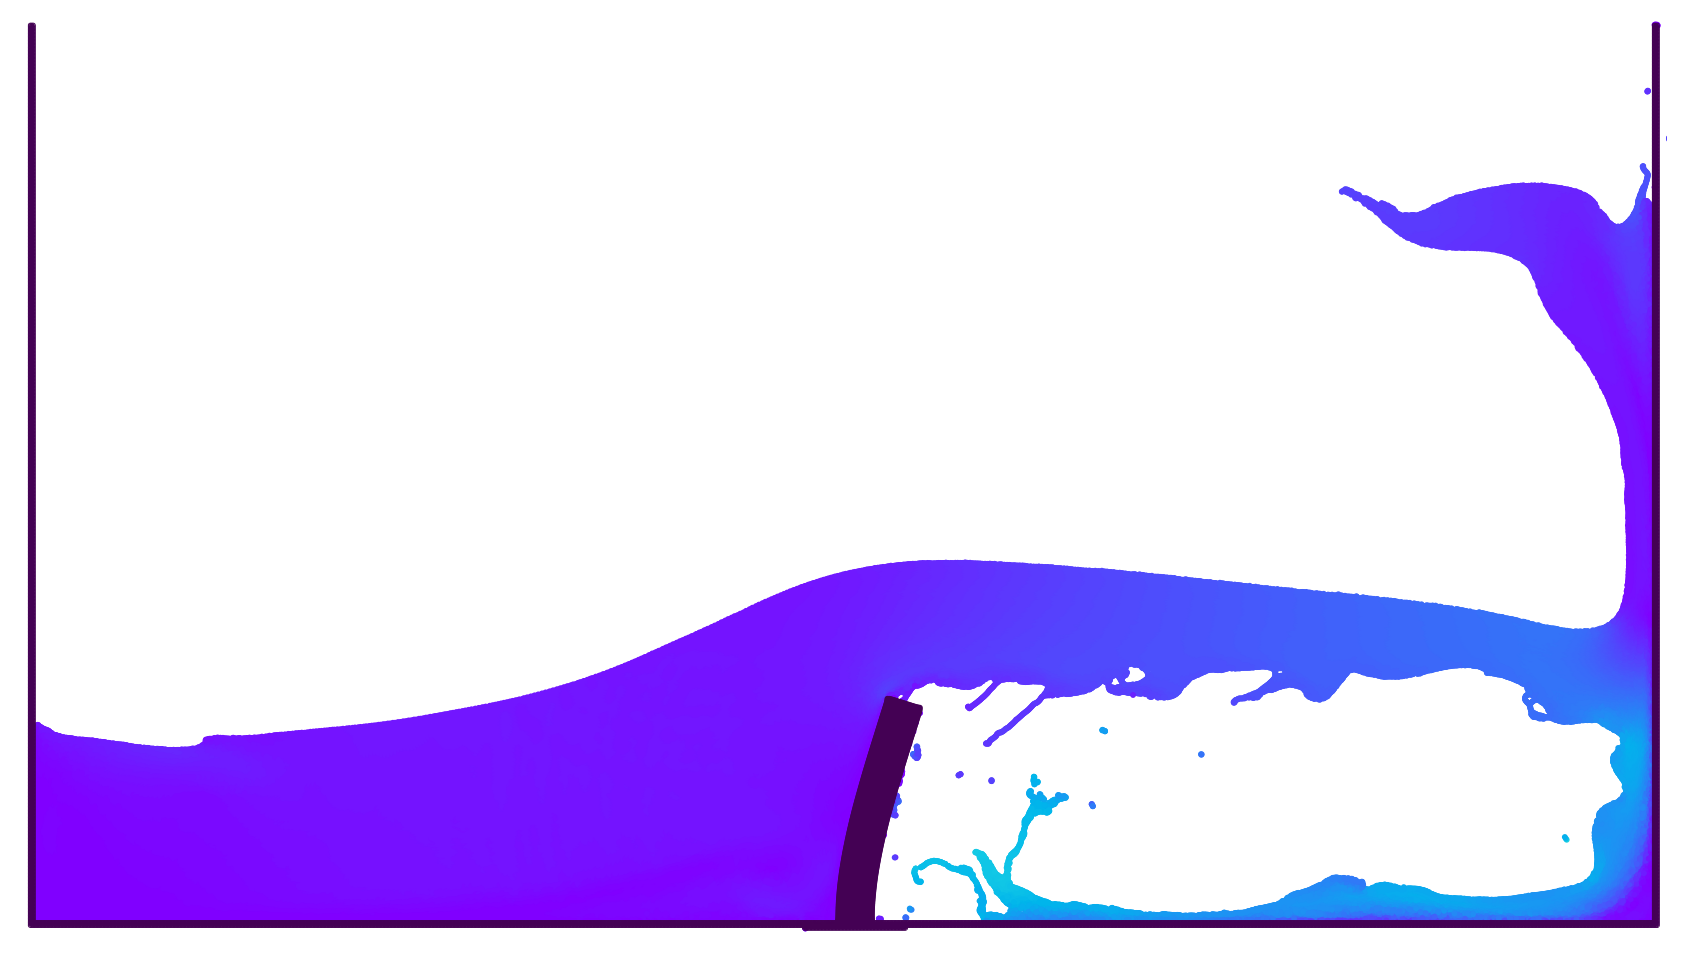
\includegraphics[scale=0.5]{figures/sun_2019_dam_breaking_flow_impacting_an_elastic_plate/snap_t_3.png}
%     }
%     \\
%     \subfigure[]
%     {
%         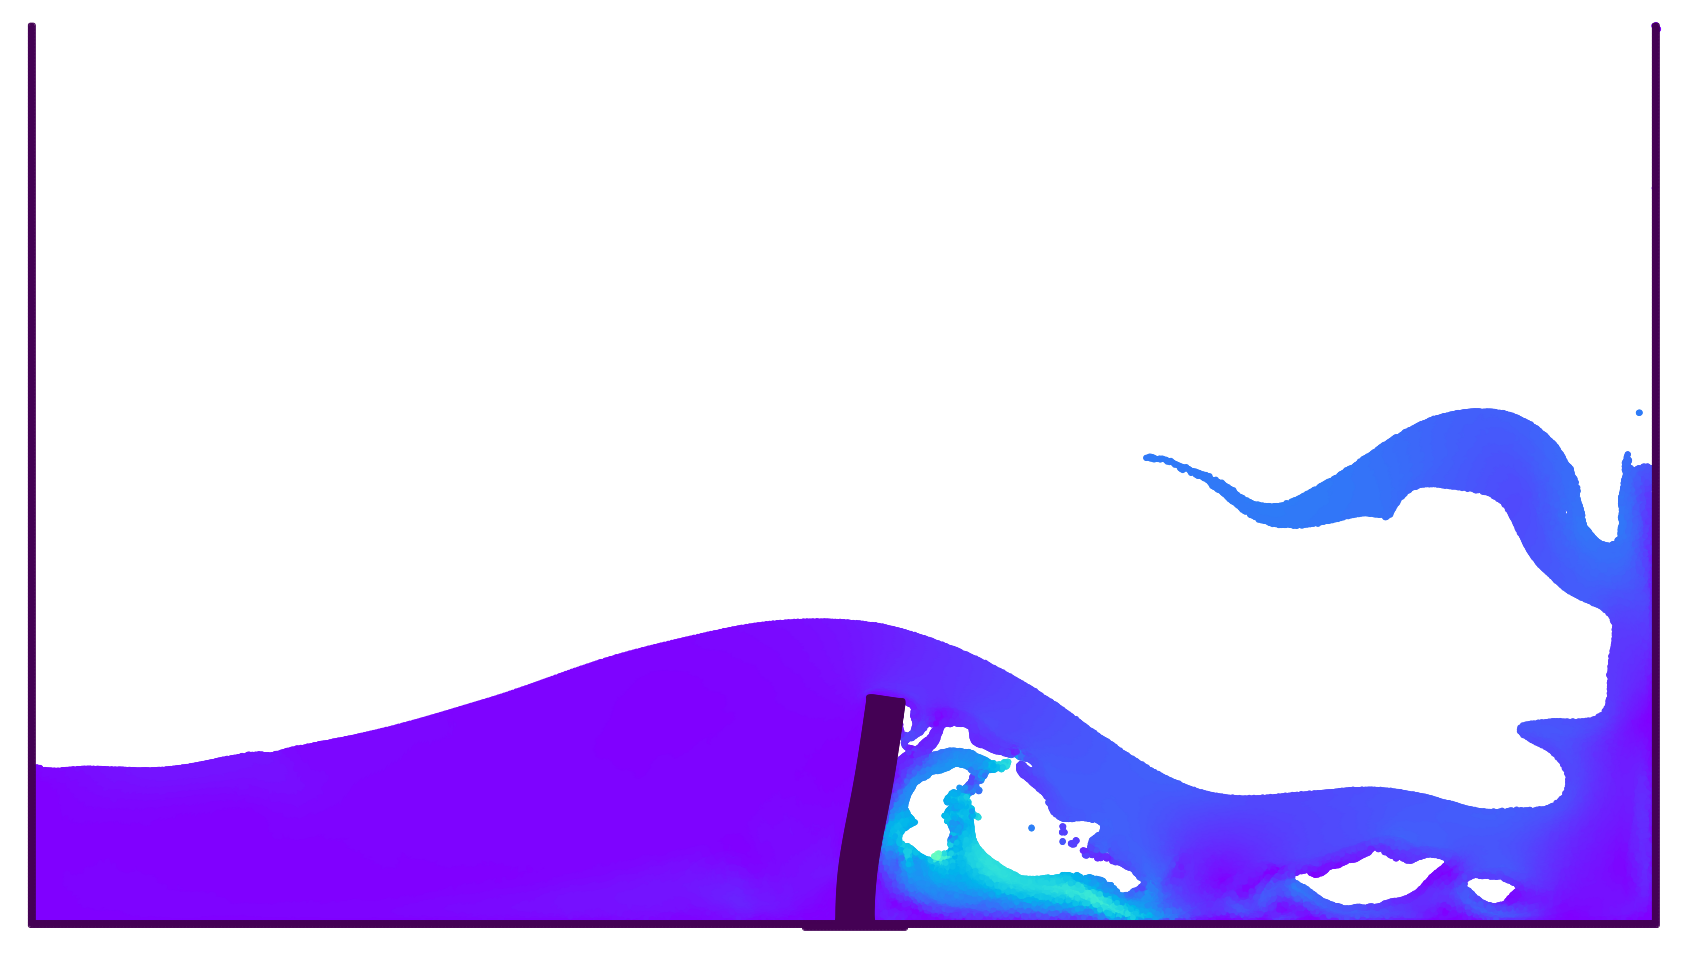
\includegraphics[scale=0.5]{figures/sun_2019_dam_breaking_flow_impacting_an_elastic_plate/snap_t_4.png}
%     }
%     \caption
%     {
%         (a) Snapshot of the fluid and the structure at different time stamps.
%     }
%     \label{fig:dam-breaking-onto-plate-snapshot}
% \end{figure}
\begin{figure}
    \centering
    \subfigure[]
    {
        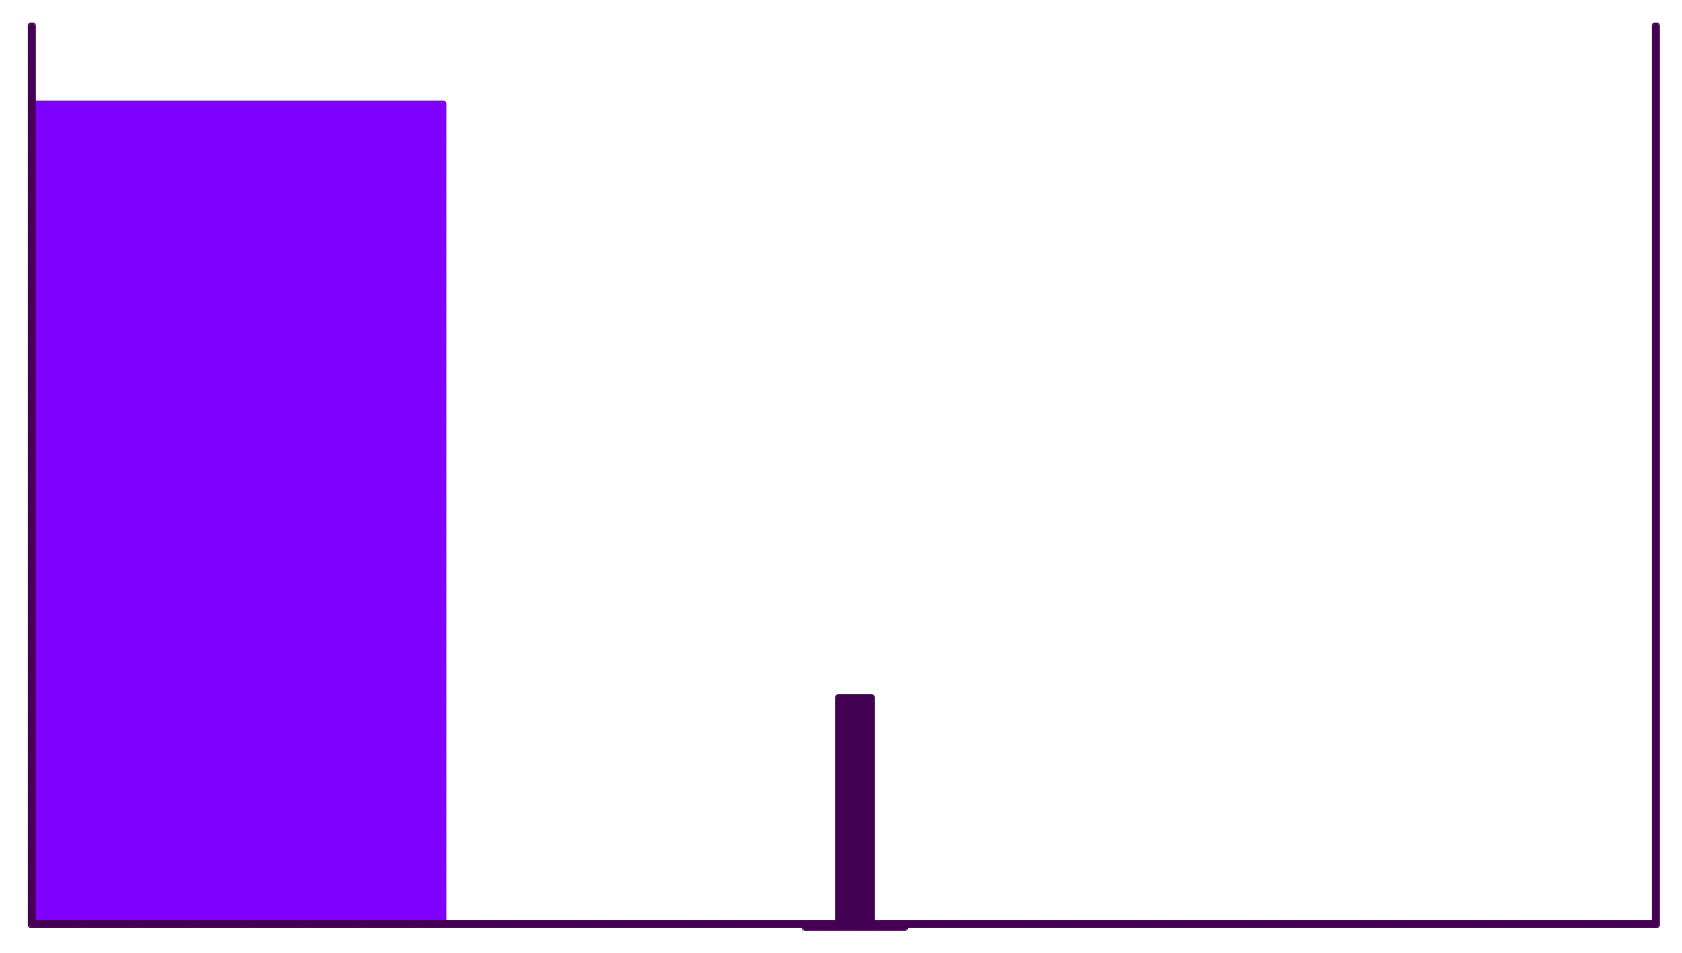
\includegraphics[scale=0.5]{figures/sun_2019_dam_breaking_flow_impacting_an_elastic_plate/snap_t_0.png}
    }
    \\
    % \subfigure[]
    % {
    %     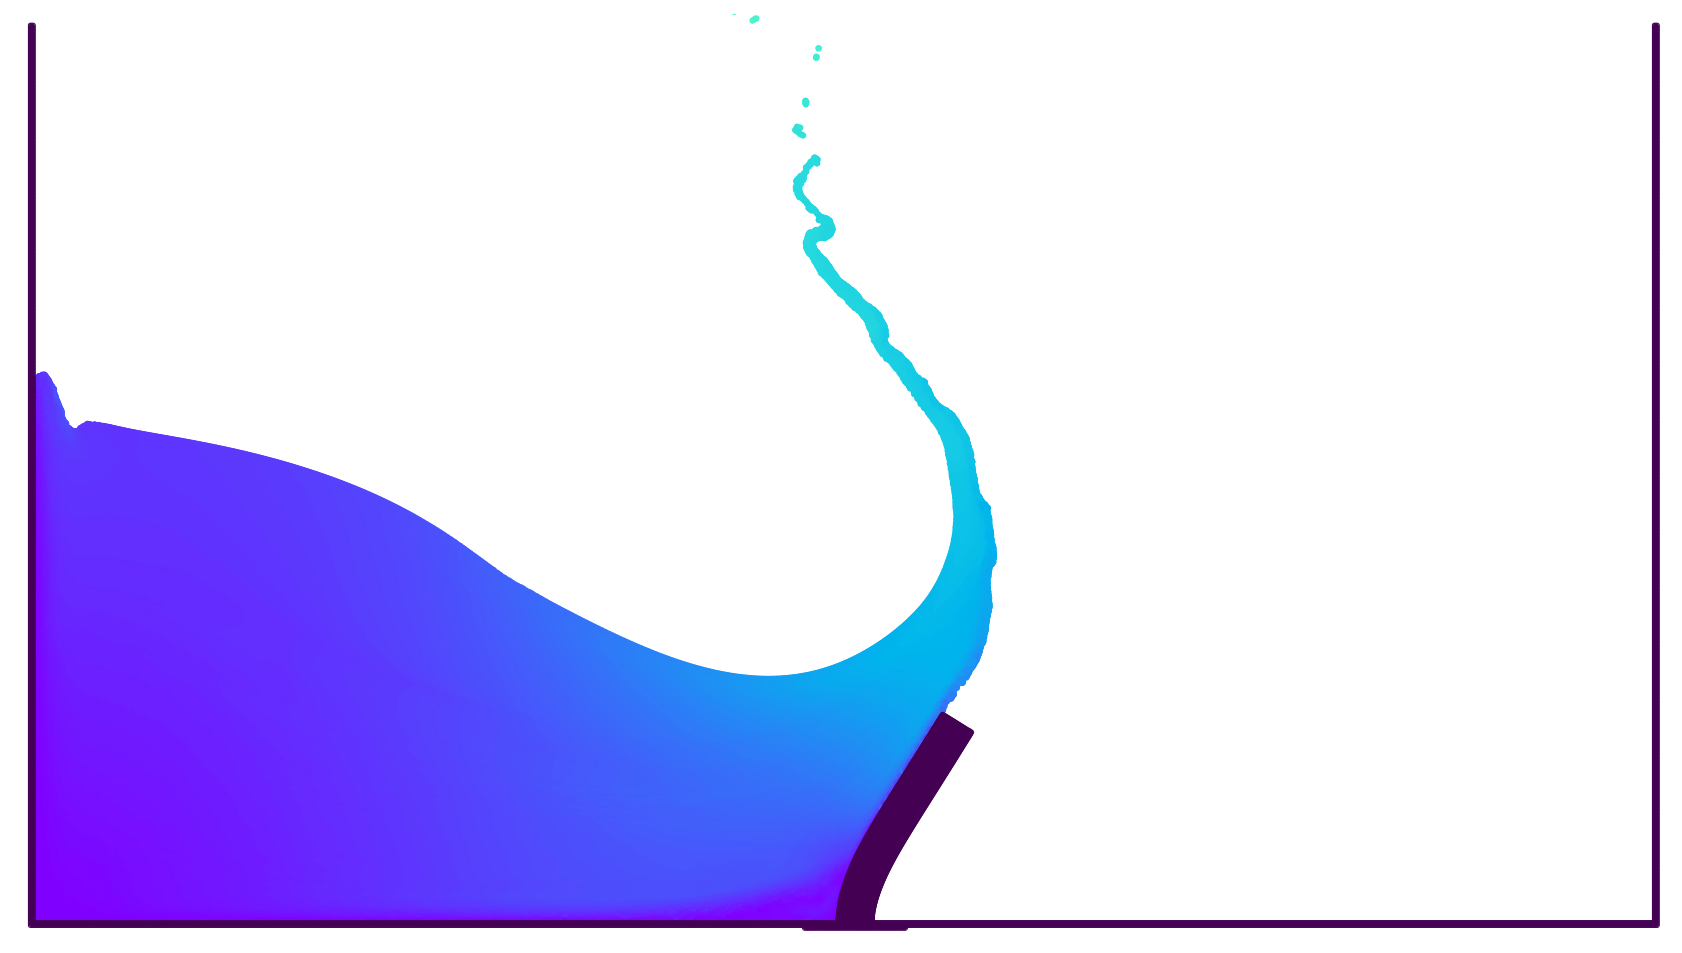
\includegraphics[scale=0.5]{figures/sun_2019_dam_breaking_flow_impacting_an_elastic_plate/snap_t_1.png}
    % }
    % \\
    \subfigure[]
    {
        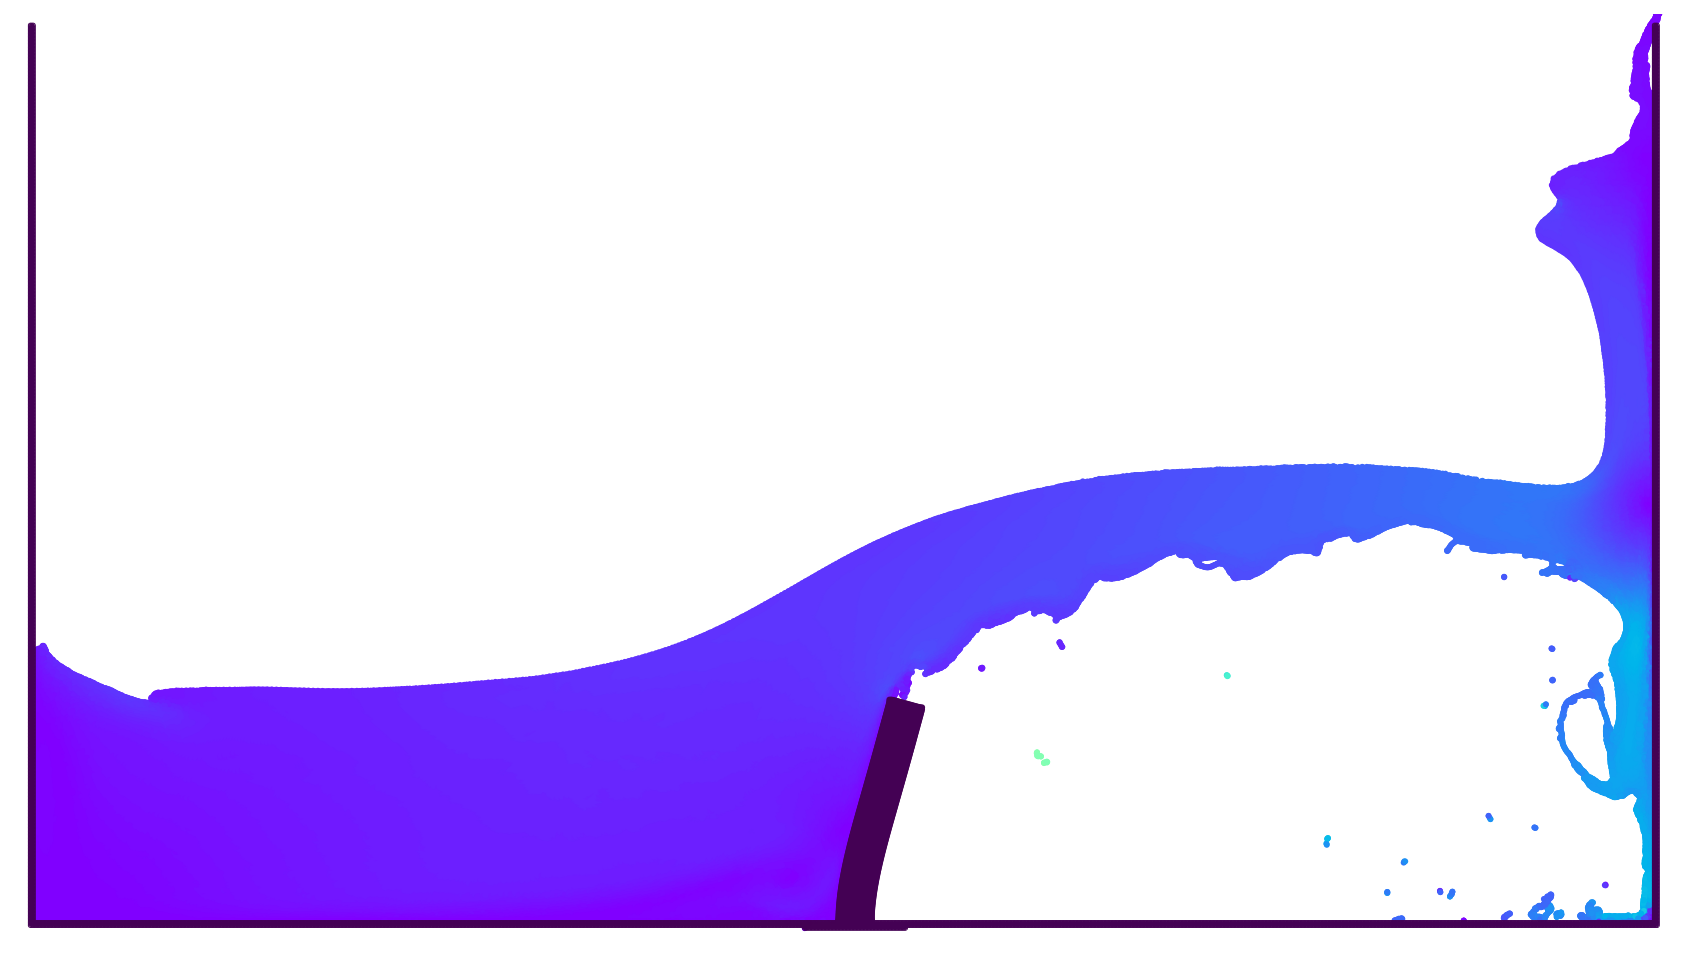
\includegraphics[scale=0.5]{figures/sun_2019_dam_breaking_flow_impacting_an_elastic_plate/snap_t_2.png}
    }
    \\
    % \subfigure[]
    % {
    %     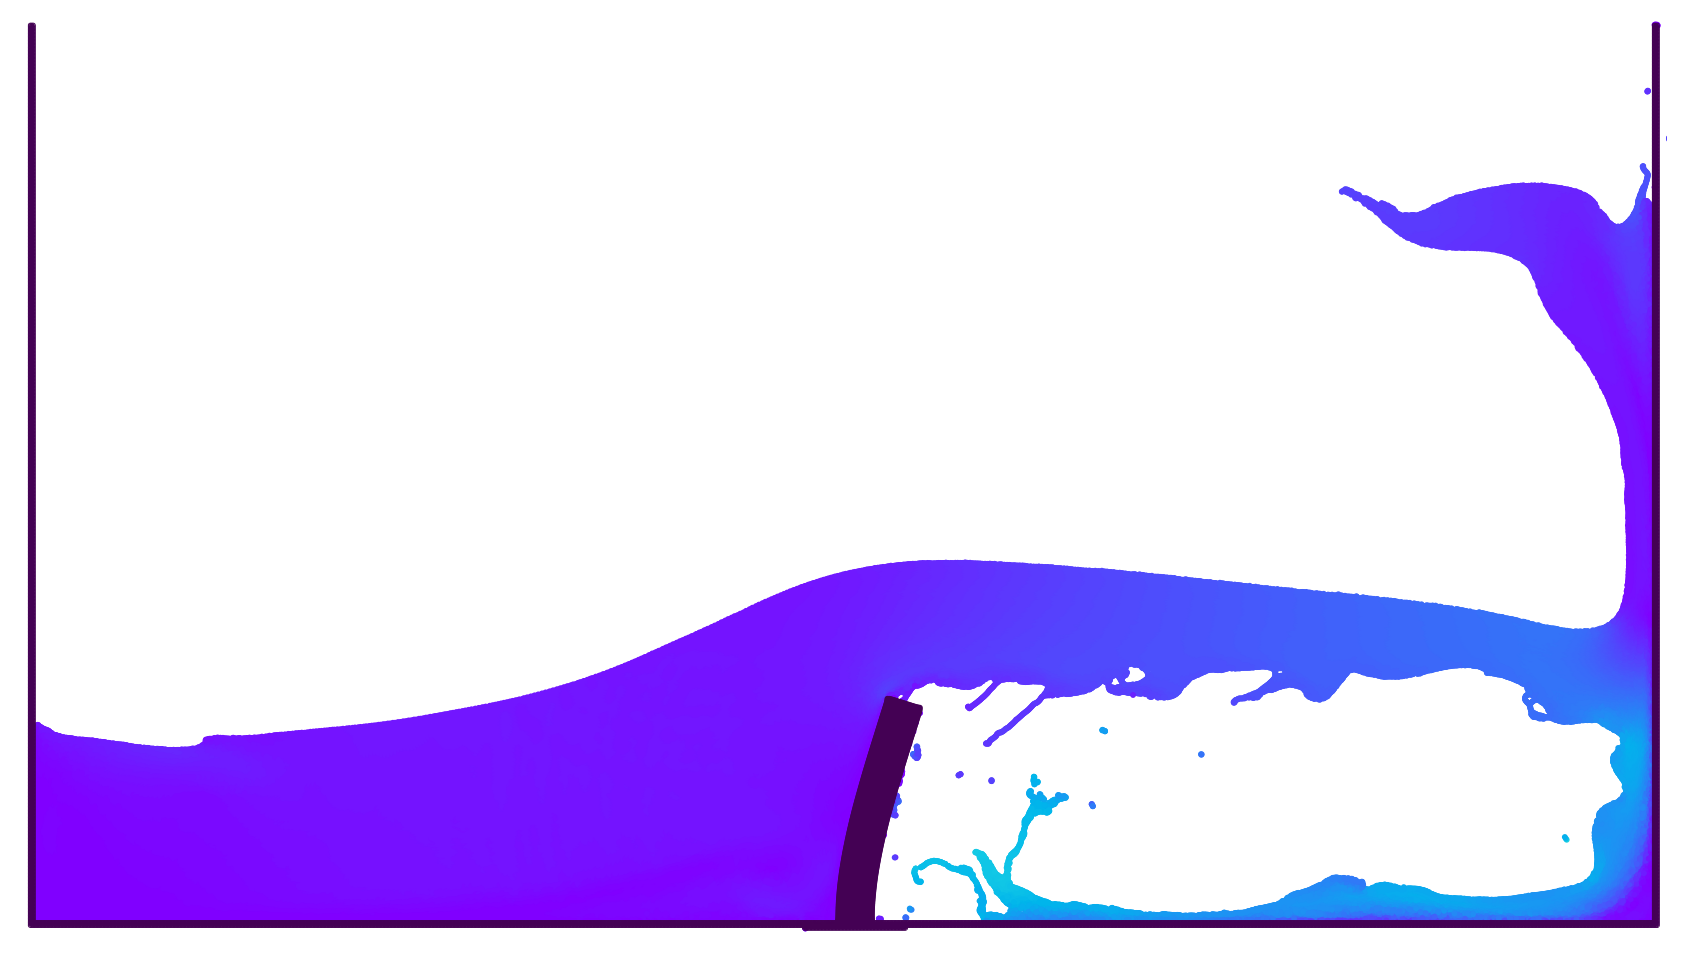
\includegraphics[scale=0.5]{figures/sun_2019_dam_breaking_flow_impacting_an_elastic_plate/snap_t_3.png}
    % }
    % \\
    \subfigure[]
    {
        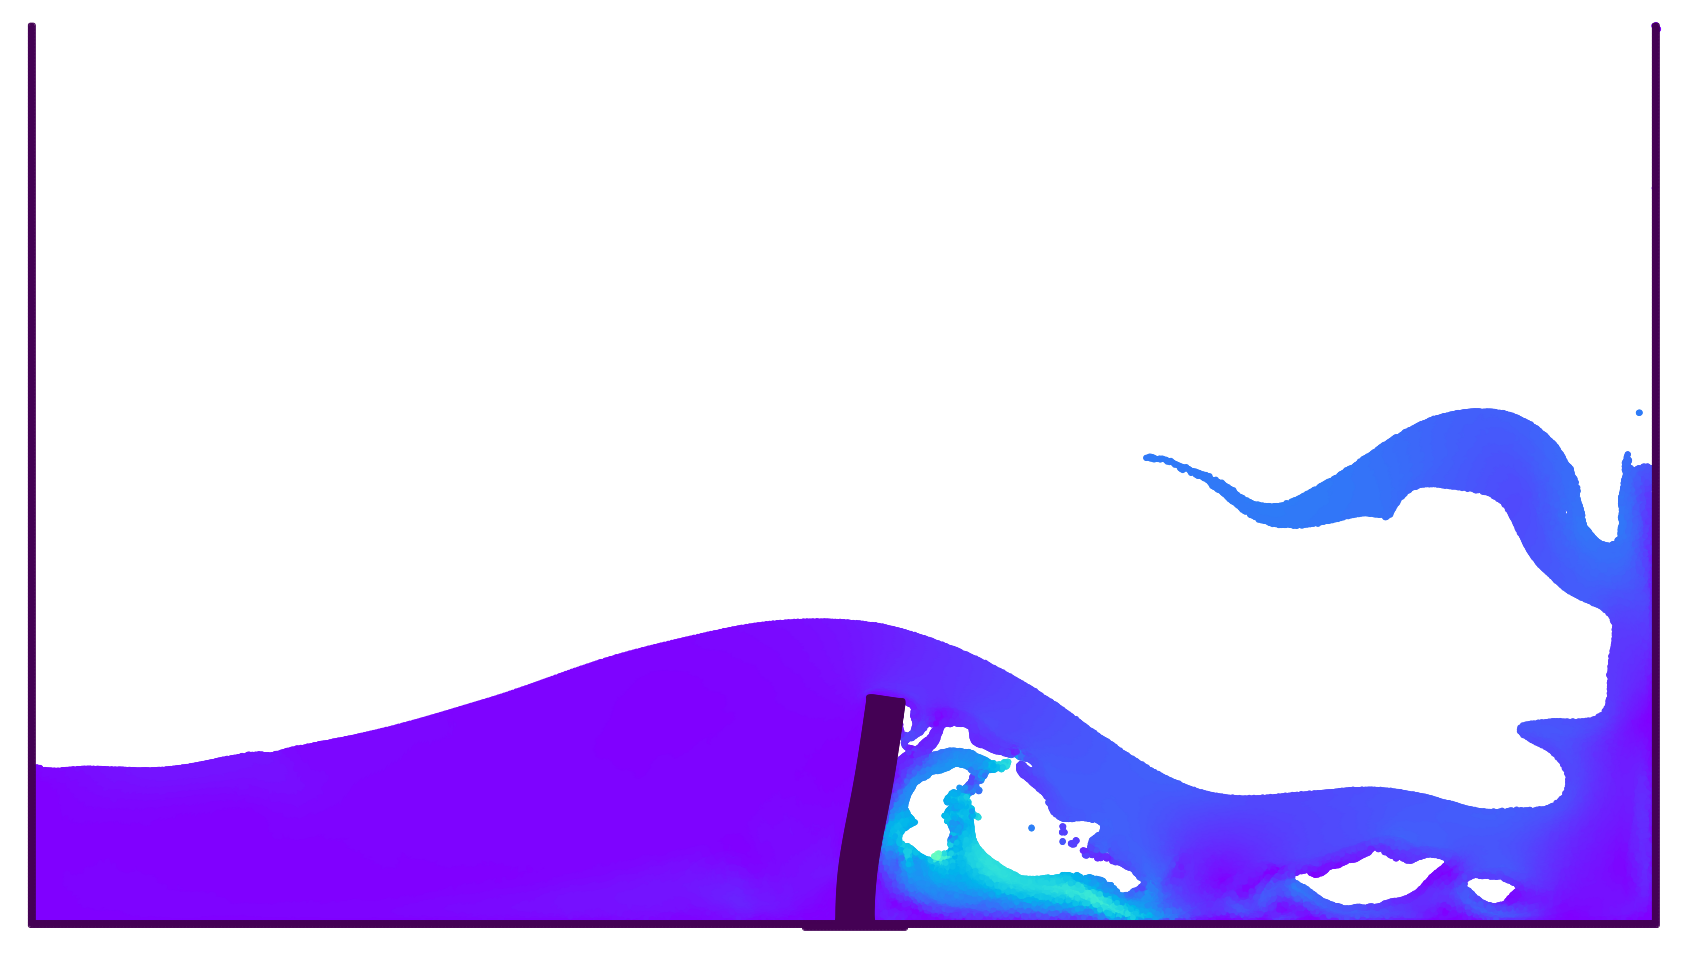
\includegraphics[scale=0.5]{figures/sun_2019_dam_breaking_flow_impacting_an_elastic_plate/snap_t_4.png}
    }
    \caption
    {
        (a) Snapshot of the fluid and the structure at different time stamps - Water impact onto an elastic plate.
    }
    \label{fig:dam-breaking-onto-plate-snapshot}
\end{figure}
\begin{figure}
  \centering
  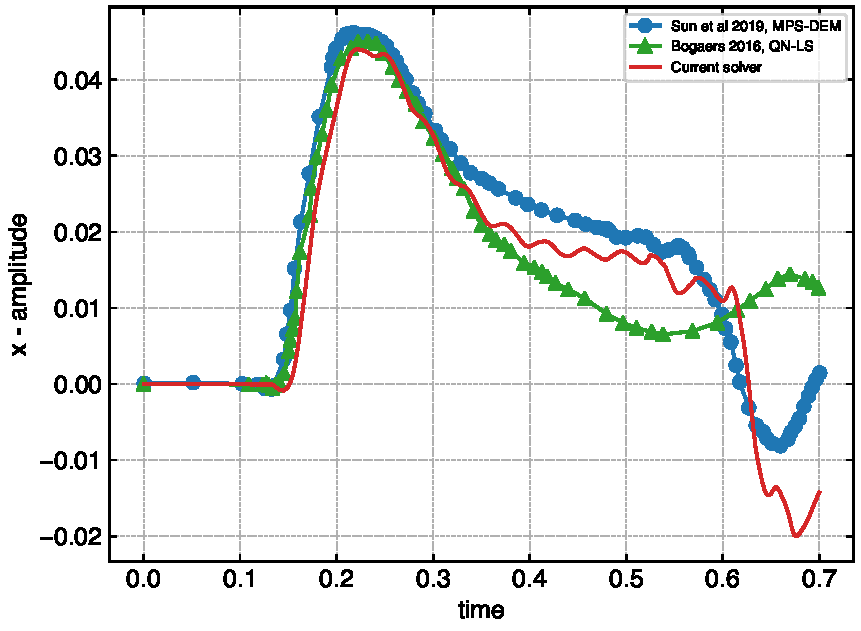
\includegraphics[scale=0.45]{figures/sun_2019_dam_breaking_flow_impacting_an_elastic_plate/x_amplitude}
  \caption{Time histories of horizontal displacement of the free end of the
    elastic structure compared against the numerical results of
    \cite{sun2019fully,bogaers2016evaluation}- Water impact onto an elastic
    plate.}
\label{fig:water-impact-plate-deflection-quantitative}
\end{figure}

% ========================================================
% ========================================================
\section{\textbf{CONCLUSIONS}}\label{sec4}
% ========================================================
% ========================================================

CTVF is able eliminate several issues SPH faces while solving fluid and solid
problems. Through particle shifting techniques as well as incorporating the
missing terms CTVF is able to produce better approxmiation in simulating fluid
problmes, also it is adaptable to different PST techniqes. Similarly with PST
the newly CTVF eliminates tensile instability while solving the elastic dynamics
probnlems. With the adavantages in mind, we solve both fluid and solid phases in
simulating FSI problems with CTVF with this approach we are able to handle FSI
problems.


We validated the current schemes by solving a UDL problem to test the structure
equations and an aluminium plate over a hydrostatic tank where an
analytical solution is available is utilized to validate the FSI part of the
current solver. The current solver is applied to wave front arising due to a dam
break hitting a steady elastic plate, here the deformation of the elastic plate
is compared against the experimental results. A convergence analysis is
undertaken for both fundamental benchmarks, UDL and hydrostatic tank.

For the future work, we plan to extend the current solver being extended to handle
the anisotropic structures and 3D FSI problems.


% \vspace{0.5cm}
% \noindent
% \textbf{ACKNOWLEDGEMENTS}\\
% % \noindent If the authors want to acknowledge any person, institute, or facilities, it may be done here. \\

% \vspace{0.5cm}
%  \noindent
% \textbf{NOMENCLATURE}\\

% \begin{tabular}{ccc}
% $A$ & Frontal area of rotor & [m$^2$]\\
% $Re$ & Reynolds number & -- \\
% $\epsilon$ & Dissipation & --
% \end{tabular}


% \cite{wu2016coupled,
% He2017coupled,
% khayyer2018enhanced,
% Sun2019study,
% zhan2019stabilized,
% wang2020scale,
% ng2020coupled,
% sun2021accurate,
% khayyer2021multi,
% long2021coupling,
% peng2021coupling,
% zhang2021deltasph,
% sun2019fully,
% hwang2014development,
% zhang2021partitioned,
% connor2021fluid,
% nasar2019flexible,
% khayyer2021coupled,
% monaghan-gingold-stars-mnras-77,
% sph:xsph:monaghan-jcp89,
% sph:fsf:monaghan-jcp94,
% zhang_hu_adams17,
% PR:pysph:scipy16,
% pysph,
% pr:automan:2018,
% monaghan-review:2005}

\bibliographystyle{amsplain}
\bibliography{references_fmfp2022}

\end{document}

%  LocalWords:  Verifications
